\documentclass[12pt,titlepage]{extarticle}
% Document Layout and Font
\usepackage{subfiles}
\usepackage[margin=2cm, headheight=15pt]{geometry}
\usepackage{fancyhdr}
\usepackage{enumitem}	
\usepackage{wrapfig}
\usepackage{float}
\usepackage{multicol}

\usepackage[p,osf]{scholax}

\renewcommand*\contentsname{Table of Contents}
\renewcommand{\headrulewidth}{0pt}
\pagestyle{fancy}
\fancyhf{}
\fancyfoot[R]{$\thepage$}
\setlength{\parindent}{0cm}
\setlength{\headheight}{17pt}
\hfuzz=9pt

% Figures
\usepackage{svg}

% Utility Management
\usepackage{color}
\usepackage{colortbl}
\usepackage{xcolor}
\usepackage{xpatch}
\usepackage{xparse}

\definecolor{gBlue}{HTML}{7daea3}
\definecolor{gOrange}{HTML}{e78a4e}
\definecolor{gGreen}{HTML}{a9b665}
\definecolor{gPurple}{HTML}{d3869b}

\definecolor{links}{HTML}{1c73a5}
\definecolor{bar}{HTML}{584AA8}

% Math Packages
\usepackage{mathtools, amsmath, amsthm, thmtools, amssymb, physics}
\usepackage[scaled=1.075,ncf,vvarbb]{newtxmath}

\newcommand\B{\mathbb{C}}
\newcommand\C{\mathbb{C}}
\newcommand\R{\mathbb{R}}
\newcommand\Q{\mathbb{Q}}
\newcommand\N{\mathbb{N}}
\newcommand\Z{\mathbb{Z}}

\DeclareMathOperator{\lcm}{lcm}

% Probability Theory
\newcommand\Prob[1]{\mathbb{P}\qty(#1)}
\newcommand\Var[1]{\text{Var}\qty(#1)}
\newcommand\Exp[1]{\mathbb{E}\qty[#1]}

% Analysis
\newcommand\ball[1]{\B\qty(#1)}
\newcommand\conj[1]{\overline{#1}}
\DeclareMathOperator{\Arg}{Arg}
\DeclareMathOperator{\cis}{cis}

% Linear Algebra
\DeclareMathOperator{\dom}{dom}
\DeclareMathOperator{\range}{range}
\DeclareMathOperator{\spann}{span}
\DeclareMathOperator{\nullity}{nullity}

% TIKZ
\usepackage{tikz}
\usepackage{pgfplots}
\usetikzlibrary{arrows.meta}
\usetikzlibrary{math}
\usetikzlibrary{cd}

% Boxes and Theorems
\usepackage[most]{tcolorbox}
\tcbuselibrary{skins}
\tcbuselibrary{breakable}
\tcbuselibrary{theorems}

\newtheoremstyle{default}{0pt}{0pt}{}{}{\bfseries}{\normalfont.}{0.5em}{}
\theoremstyle{default}

\renewcommand*{\proofname}{\textit{\textbf{Proof.}}}
\renewcommand*{\qedsymbol}{$\blacksquare$}
\tcolorboxenvironment{proof}{
	breakable,
	coltitle = black,
	colback = white,
	frame hidden,
	boxrule = 0pt,
	boxsep = 0pt,
	borderline west={3pt}{0pt}{bar},
	% borderline west={3pt}{0pt}{gPurple},
	sharp corners = all,
	enhanced,
}

\newtheorem{theorem}{Theorem}[section]{\bfseries}{}
\tcolorboxenvironment{theorem}{
	breakable,
	enhanced,
	boxrule = 0pt,
	frame hidden,
	coltitle = black,
	colback = blue!7,
	% colback = gBlue!30,
	left = 0.5em,
	sharp corners = all,
}

\newtheorem{corollary}{Corollary}[section]{\bfseries}{}
\tcolorboxenvironment{corollary}{
	breakable,
	enhanced,
	boxrule = 0pt,
	frame hidden,
	coltitle = black,
	colback = white!0,
	left = 0.5em,
	sharp corners = all,
}

\newtheorem{lemma}{Lemma}[section]{\bfseries}{}
\tcolorboxenvironment{lemma}{
	breakable,
	enhanced,
	boxrule = 0pt,
	frame hidden,
	coltitle = black,
	colback = green!7,
	left = 0.5em,
	sharp corners = all,
}

\newtheorem{definition}{Definition}[section]{\bfseries}{}
\tcolorboxenvironment{definition}{
	breakable,
	coltitle = black,
	colback = white,
	frame hidden,
	boxsep = 0pt,
	boxrule = 0pt,
	borderline west = {3pt}{0pt}{orange},
	% borderline west = {3pt}{0pt}{gOrange},
	sharp corners = all,
	enhanced,
}

\newtheorem{example}{Example}[section]{\bfseries}{}
\tcolorboxenvironment{example}{
	% title = \textbf{Example},
	% detach title,
	% before upper = {\tcbtitle\quad},
	breakable,
	coltitle = black,
	colback = white,
	frame hidden,
	boxrule = 0pt,
	boxsep = 0pt,
	borderline west={3pt}{0pt}{green!70!black},
	% borderline west={3pt}{0pt}{gGreen},
	sharp corners = all,
	enhanced,
}

\newtheoremstyle{remark}{0pt}{4pt}{}{}{\bfseries\itshape}{\normalfont.}{0.5em}{}
\theoremstyle{remark}
\newtheorem*{remark}{Remark}


% TColorBoxes
\newtcolorbox{week}{
	colback = black,
	coltext = white,
	fontupper = {\large\bfseries},
	width = 1.2\paperwidth,
	size = fbox,
	halign upper = center,
	center
}

\newcommand{\banner}[2]{
    \pagebreak
    \begin{week}
   		\section*{#1}
    \end{week}
    \addcontentsline{toc}{section}{#1}
    \addtocounter{section}{1}
    \setcounter{subsection}{0}
}

% Hyperref
\usepackage{hyperref}
\hypersetup{
	colorlinks=true,
	linktoc=all,
	linkcolor=links,
	bookmarksopen=true
}

% Error Handling
\PackageWarningNoLine{ExtSizes}{It is better to use one of the extsizes 
                          classes,^^J if you can}


\def\homeworknumber{1}
\fancyhead[R]{\textbf{Math 140A: Homework \#\homeworknumber}}
\fancyhead[L]{Eli Griffiths}
\renewcommand{\headrulewidth}{1pt}
\setlength\parindent{0pt}


\usepackage{truthtable}
\usepackage{pifont}
\usepackage{pdfpages}

\begin{document}

\subsection*{1.1.1}
The propositions are a through d and all are true except d.

\subsection*{1.1.5}
\begin{tasks}(2)
    \task Mei does not have an MP3 player
    \task There is pollution in New Jersey
    \task $2 + 1 \neq 3$
    \task The summer in Maine is not hot or it is not sunny
\end{tasks}

\subsection*{1.1.9}

% Acme    138 8
% Nadir   87  5
% Quixote 111 13
%

\begin{tasks}(3)
    \task False
    \task $T \land T \equiv$ True
    \task $F \lor T \equiv$ True
    \task  $F \rightarrow T \equiv$ True
    \task $T \leftrightarrow T \equiv$ True
\end{tasks}

\subsection*{1.1.11}
\begin{tasks}(2)
    \task Sharks have not been spotted near the shore
    \task Swimming at the New Jersey shore is allowed and sharks have been spotted near the shore
    \task Swimming at the New Jersey shore is not allowed, or sharks have been spotted near the shore
    \task If swimming is allowed at the New Jersey shore, then sharks have not been spotted at the shore
    \task If sharks have not been spotted at the New Jersey shore, then swimming is allowed at the shore
    \task If swimming is not allowed at the New Jersey shore, then sharks have not been spotted at the shore
    \task Swimming at the New Jersey shore is allowed if and only if no sharks have been spotted at the shore
    \task Swimming at the New Jersey shore is not allowed, and either swimming at the shore is allowed or sharks have not been spotted near the shore
\end{tasks}

\subsection*{1.1.13}
\begin{tasks}(3)
    \task $p \land q$
    \task $p \land \lnot q$
    \task $\lnot p \land \lnot q$
    \task $p \lor q$
    \task $p \rightarrow q$
    \task $(p \lor q) \land (p \rightarrow \lnot q)$
    \task $q \leftrightarrow p$
\end{tasks}

\subsection*{1.1.19}
\begin{tasks}(2)
    \task $T \rightarrow F \equiv$ False
    \task $F \rightarrow T \equiv$ True
    \task $F \rightarrow F \equiv$ True
    \task $F \rightarrow F \equiv$ True
\end{tasks}

\subsection*{1.1.27}
\begin{tasks}(2)
    \task It is hot outside if and only if you buy an ice cream cone
    \task You win the contest if and only if you have the only winning ticket
    \task You get promoted if and only if you have connections
    \task Your mind will decay if and only if you watch television
    \task The trains run late if and only if its a day I take them
\end{tasks}

\subsection*{1.1.29}

\begin{problem}
    \begin{enumerate}[leftmargin=3.0cm]
        \item[Converse)] If I ski tomorrow, it will have snowed today
        \item[Contrapositive)] If I don't ski tomorrow, then it didn't snow today
        \item[Inverse)] If it doesn't snow today, then I won't ski tomorrow
    \end{enumerate}
\end{problem}

\begin{problem}
    \begin{enumerate}[leftmargin=3cm]
        \item[Converse)] If I come to class, then there was going to be a quiz
        \item[Contrapositive)] If there isn't a quiz in class, then I wont come
        \item[Inverse)] If there isn't going to be a quiz in class, then I wont come
    \end{enumerate}
\end{problem}

\begin{problem}
    \begin{enumerate}[leftmargin=3cm]
        \item[Converse)] If a positive integer has no divisors other than 1 and itself, then it is prime
        \item[Contrapositive)] If a positive integer has divisors other than 1 and itself, then it is not prime
        \item[Inverse)] A positive integer is not prime only if it has divisors other than 1 and itself
    \end{enumerate}
\end{problem}


\subsection*{1.1.33}

\begin{tasks}
    \task\begin{tabular}{c||c|c}
        \truthtable{p}{$p$}{!p, p & !p}{$\lnot p$, $p \land \lnot p$}{T}{F}
    \end{tabular}

    \task\begin{tabular}{c||c|c}
        \truthtable{p}{$p$}{!p, p | !p}{$\lnot p$, $p \lor \lnot p$}{T}{F}
    \end{tabular}

    \task\begin{tabular}{c|c||c|c|c}
        \truthtable{p,q}{$p$, $q$}{!q, p | !q, >>((p | !q); q)}{$\lnot q$, $p \lor \lnot q$, $(p \lor \lnot q) \rightarrow q$}{T}{F}
    \end{tabular}

    \task\begin{tabular}{c|c||c|c|c}
        \truthtable{p,q}{$p$, $q$}{p | q, p & q, >>(p | q; p & q)}{$p \lor q$, $p \land q$, $(p \lor q) \rightarrow (p \land q)$}{T}{F}
    \end{tabular}

    \task\begin{tabular}{c|c||c|c|c|c|c}
        \truthtable{p,q}{$p$, $q$}{!p, !q, >>(p; q), >>(!q; !p), <>(>>(p; q); >>(!q; !p))}{$\lnot p$, $\lnot q$, $p \rightarrow q$, $\lnot q \rightarrow \lnot p$, $(p \rightarrow q) \leftrightarrow (\lnot q \rightarrow \lnot p)$}{T}{F}
    \end{tabular}
    \task\begin{tabular}{c|c||c|c|c}
        \truthtable{p,q}{$p$, $q$}{>>(p; q), >>(q; p), >>(>>(p; q); >>(q; p))}{$p \rightarrow q$, $q \rightarrow p$, $(p \rightarrow q) \rightarrow (q \rightarrow p)$}{T}{F}
    \end{tabular}
\end{tasks}


\subsection*{1.1.39}
\begin{tasks}
    \task\begin{tabular}{c|c||c|c|c|c}
        \truthtable{p,q,r}{$p$, $q$, $r$}{!q, !q | r, >>(p; !q | r)}{$\lnot q$, $\lnot q \lor r$, $p \rightarrow (\lnot q \lor r)$}{T}{F}
    \end{tabular}

    \task\begin{tabular}{c|c||c|c|c|c}
        \truthtable{p,q,r}{$p$, $q$, $r$}{!p, >>(q;r), >>(!p; >>(q;r))}{$\lnot p$, $q \rightarrow r$, $\lnot p \rightarrow (q \rightarrow r)$}{T}{F}
    \end{tabular}

    \task\begin{tabular}{c|c||c|c|c|c|c}
        \truthtable{p,q,r}{$p$, $q$, $r$}{!p, >>(p;q), >>(!p; r), >>(p;q) | >>(!p;r)}{$\lnot p$, $p \rightarrow q$, $\lnot p \rightarrow r$, $(p \rightarrow q) \lor (\lnot p \rightarrow r)$}{T}{F}
    \end{tabular}

    \task\begin{tabular}{c|c||c|c|c|c|c}
        \truthtable{p,q,r}{$p$, $q$, $r$}{!p, >>(p;q), >>(!p; r), >>(p;q) & >>(!p;r)}{$\lnot p$, $p \rightarrow q$, $\lnot p \rightarrow r$, $(p \rightarrow q) \land (\lnot p \rightarrow r)$}{T}{F}
    \end{tabular}

    \task\begin{tabular}{c|c||c|c|c|c|c}
        \truthtable{p,q,r}{$p$, $q$, $r$}{!q, <>(p;q), <>(!q; r), <>(p;q) | <>(!q;r)}{$\lnot q$, $p \leftrightarrow q$, $\lnot q \leftrightarrow r$, $(p \leftrightarrow q) \lor (\lnot q \leftrightarrow r)$}{T}{F}
    \end{tabular}

    \task\begin{tabular}{c|c||c|c|c|c|c|c}
        \truthtable{p,q,r}{$p$, $q$, $r$}{!p, !q, <>(!p;!q), <>(q;r), <>(<>(!p;!q);<>(q;r))}{$\lnot p$, $\lnot q$, $\lnot p \leftrightarrow \lnot q$, $q \leftrightarrow r$, $(\lnot p \leftrightarrow \lnot q) \leftrightarrow (q \leftrightarrow r)$}{T}{F}
    \end{tabular}
\end{tasks}

\subsection*{1.2.5}
\[
    e \rightarrow (a \land (b \lor p) \land r)
.\]

\subsection*{1.2.29}
Let $K$ denote being a knight, $k$ denote being the knave, and $s$ the spy.

\newcommand{\Yes}{\ding{51}}
\newcommand{\Noo}{\ding{55}}

\begin{center}
    \begin{tabular}{c|c|c||c|c|c||c}
        A & B & C       & T(A) & T(B) & T(C) & Possible? \\\hline
        $K$ & $k$ & $s$ & \Yes & \Noo & \Yes & \Noo \\\hline
        $K$ & $s$ & $k$ & \Yes & \Yes & \Yes & \Yes \\\hline
        $k$ & $K$ & $s$ & \Yes & \Noo & \Yes & \Noo \\\hline
        $s$ & $K$ & $k$ & \Yes & \Noo & \Noo & \Noo \\\hline
        $k$ & $s$ & $K$ & \Yes & \Yes & \Noo & \Noo \\\hline
        $s$ & $k$ & $K$ & \Yes & \Noo & \Noo & \Noo
    \end{tabular}
\end{center}

\subsection*{1.2.31}

\begin{center}
    \begin{tabular}{c|c|c||c|c|c||c}
        A & B & C       & T(A) & T(B) & T(C) & Possible? \\\hline
        $K$ & $k$ & $s$ & \Yes & \Noo & \Yes & \Noo \\\hline
        $K$ & $s$ & $k$ & \Yes & \Yes & \Yes & \Yes \\\hline
        $k$ & $K$ & $s$ & \Yes & \Noo & \Yes & \Noo \\\hline
        $s$ & $K$ & $k$ & \Yes & \Noo & \Yes & \Noo \\\hline
        $k$ & $s$ & $K$ & \Yes & \Yes & \Noo & \Noo \\\hline
        $s$ & $k$ & $K$ & \Yes & \Yes & \Noo & \Noo
    \end{tabular}
\end{center}

\subsection*{1.2.33}

\begin{center}
    \begin{tabular}{c|c|c||c|c|c||c}
        A & B & C       & T(A) & T(B) & T(C) & Possible? \\\hline
        $K$ & $k$ & $s$ & \Yes & \Yes & \Yes & \Yes \\\hline
        $K$ & $s$ & $k$ & \Yes & \Yes & \Yes & \Yes \\\hline
        $k$ & $K$ & $s$ & \Yes & \Yes & \Yes & \Yes \\\hline
        $s$ & $K$ & $k$ & \Yes & \Yes & \Yes & \Yes \\\hline
        $k$ & $s$ & $K$ & \Yes & \Yes & \Yes & \Yes \\\hline
        $s$ & $k$ & $K$ & \Yes & \Yes & \Yes & \Yes
    \end{tabular}
\end{center}

\subsection*{1.2.35}

\begin{center}
    \begin{tabular}{c|c|c||c|c|c||c}
        A & B & C       & T(A) & T(B) & T(C) & Possible? \\\hline
        $K$ & $k$ & $s$ & \Yes & \Noo & \Yes & \Noo \\\hline
        $K$ & $s$ & $k$ & \Yes & \Yes & \Noo & \Noo \\\hline
        $k$ & $K$ & $s$ & \Noo & \Yes & \Yes & \Noo \\\hline
        $s$ & $K$ & $k$ & \Yes & \Yes & \Noo & \Noo \\\hline
        $k$ & $s$ & $K$ & \Noo & \Yes & \Yes & \Noo \\\hline
        $s$ & $k$ & $K$ & \Yes & \Noo & \Yes & \Noo
    \end{tabular}
\end{center}

\subsection*{1.2.45}
\[
    \lnot (p \land (q \lor \lnot r))
.\]

\subsection*{1.2.47}

\begin{center}
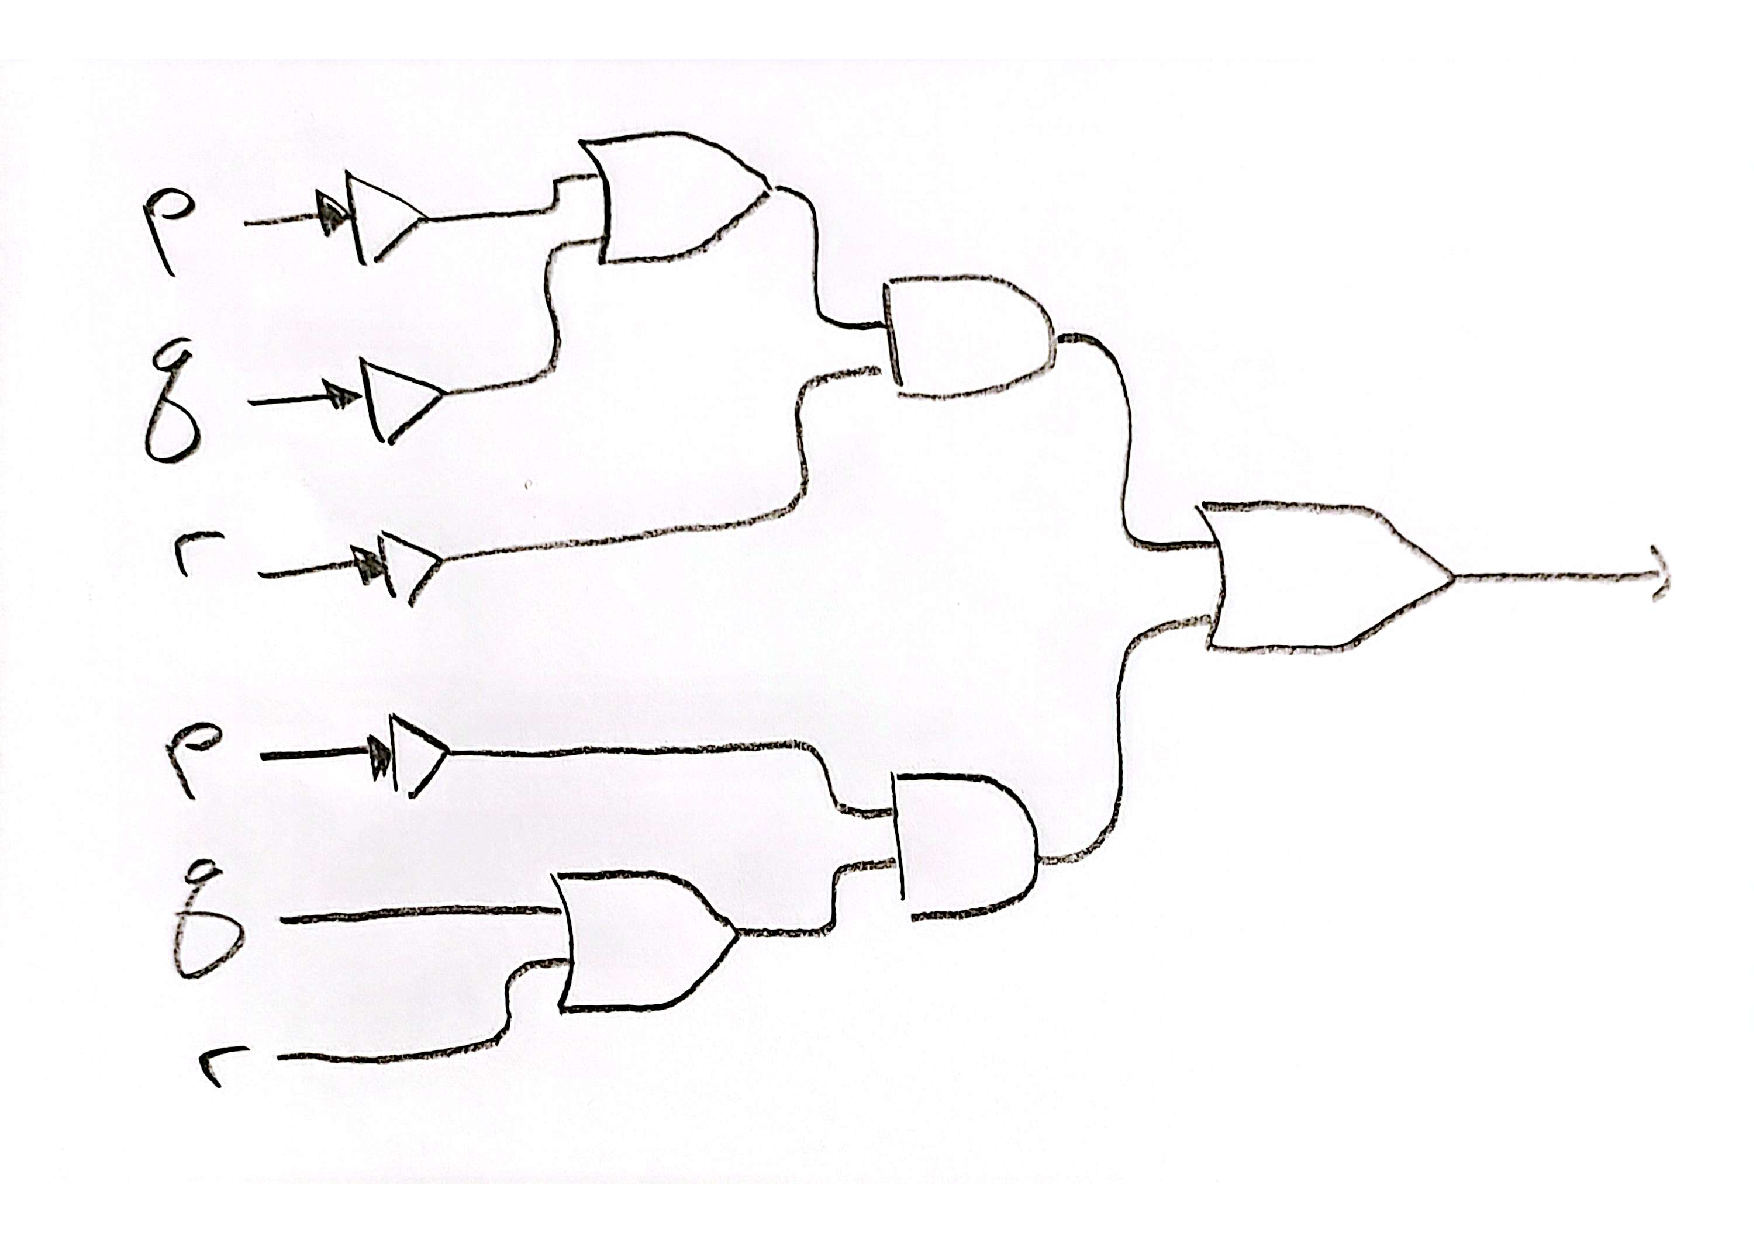
\includegraphics[scale=0.25]{circuit.pdf}
\end{center}

\subsection*{1.3.1}

\begin{tasks}(3)
    \task\begin{tabular}{c||c||c}
        $p$ & $p \land \mathbf{T}$ & p \\\hline
        T & T & T \\\hline
        F & F & F
    \end{tabular}

    \task\begin{tabular}{c||c||c}
        $p$ & $p \land \mathbf{F}$ & $\mathbf{F}$ \\\hline
        T & F & F \\\hline
        F & F & F
    \end{tabular}

    \task\begin{tabular}{c||c||c}
        $p$ & $p \lor p$ & $p$ \\\hline
        T & T & T \\\hline
        F & F & F
    \end{tabular}

    \task\begin{tabular}{c||c||c}
        $p$ & $p \lor \mathbf{F}$ & $p$ \\\hline
        T & T & T \\\hline
        F & F & F
    \end{tabular}

    \task\begin{tabular}{c||c||c}
        $p$ & $p \lor \mathbf{T}$ & $\mathbf{T}$ \\\hline
        T & T & T \\\hline
        F & T & T
    \end{tabular}

    \task\begin{tabular}{c||c||c}
        $p$ & $p \land p$ & $p$ \\\hline
        T & T & T \\\hline
        F & F & F
    \end{tabular}
\end{tasks}

\subsection*{1.3.7}
\begin{tasks}(2)
    \task\begin{tabular}{c|c||c||c}
        $p$ & $q$ & $p \lor q$ & $q \lor p$ \\\hline
        T & T & T & T \\\hline
        T & F & T & T \\\hline
        F & T & T & T \\\hline
        F & F & F & F
    \end{tabular}

    \task\begin{tabular}{c|c||c||c}
        $p$ & $q$ & $p \land q$ & $q \land p$ \\\hline
        T & T & T & T \\\hline
        T & F & F & F \\\hline
        F & T & F & F \\\hline
        F & F & F & F
    \end{tabular}
\end{tasks}

\subsection*{1.3.13}
\begin{tasks}
    \task For the implication to be false, $p \land q$ must be true and $p$ false. However is $p \land q$ is true, then $p$ is also true and therefore $p$ cannot be false. Hence it is a tautology
    \task For the implication to be false, $p$ must be true and $p \lor q$ false. However, since $p$ is true, $p \lor q$ must be true and hence this case isnt possible. Hence it is a tautology
    \task For the implication to be false, $\lnot p$ must be true and $p \to q$ must be false. Since $\lnot p$ is true, $p$ is false and therefore $p \to q$ is true meaning this case isn't possible. Hence it is a tautology
    \task For the implication to be false, $p \land q$ must be true and $p \to q$ must be false. Since $p \land q$ is true, both $p$ and $q$ must be true and therefore $p \to q$ is true. Therefore this case isn't possible meaning it is a tautology
    \task For the implication to be false, $\lnot (p \to q)$ must be true and $p$ false. Since $p$ is false, $p \to q$ is true and hence $\lnot (p \to q)$ is false. Therefore this case isn't possible meaning it is a tautology
    \task For the implication to be false, $\lnot (p \to q)$ must be true and $\lnot q$ be false. Since $\lnot q$ is false, $q$ is true meaning $p \to q$ is true regardless of $p$. Therefore $\lnot (p \to q)$ is false meaning this case isn't possible. Hence it is a tautology
\end{tasks}

\subsection*{1.3.21}
Two propositions are logically equivalent when they both are true given the exact same inputs. Since both are only true when $p$ and $q$ are of opposite truth, they are logically equivalent.

\subsection*{1.3.27}
Two propositions are logically equivalent when they both are false given the exact same inputs. The left side is false when either of the conditionals are false. This is the case only when $r$ is false and one of $p$ or $q$ is true. But that means $p \lor q$ is true and therefore the right side is also false. This is the only situation in which the right is false, therefore the propositions are logically equivalent.

\subsection*{1.3.33}
\begin{center}
    \begin{tabular}{c|c|c||c|c|c|c|c}
        \truthtable{p,q,r}{$p$, $q$, $r$}{>>(p;q), >>(q;r), >>(p;r), >>(p;q) & >>(q;r), >>(>>(p;q) & >>(q;r); >>(p; r))}{$p \rightarrow q$, $q \rightarrow r$, $p \rightarrow r$, $(p \rightarrow q) \land (q \rightarrow r)$, $(p \rightarrow q) \land (q \rightarrow r) \rightarrow (p \rightarrow r)$}{T}{F}
    \end{tabular}
\end{center}

\subsection*{1.4.1}
\begin{tasks}(3)
    \task True
    \task True
    \task False
\end{tasks}

\subsection*{1.4.5}
\begin{tasks}
    \task There is a student that spends more than five hours every weekday in class
    \task Every student spends more than five hours every weekday in class
    \task There is a student that does not spend more than five hours every weekday in class
    \task Every student does not spend more than five hours every weekday in class
\end{tasks}

\subsection*{1.4.7}
\begin{tasks}
    \task All comedians are funny
    \task Everyone is a funny comedian
    \task There is a person who if they're comedian, they are funny
    \task There is a funny comedian
\end{tasks}

\subsection*{1.4.11}
\begin{tasks}(3)
    \task True
    \task True
    \task False
    \task False
    \task True
    \task False
\end{tasks}

\subsection*{1.4.17}
\begin{tasks}(2)
    \task $P(0) \lor P(1) \lor P(2) \lor P(3) \lor P(4)$
    \task $P(0) \land P(1) \land P(2) \land P(3) \land P(4)$
    \task $\lnot P(0) \lor \lnot P(1) \lor \lnot P(2) \lor \lnot P(3) \lor \lnot P(4)$
    \task $\lnot P(0) \land \lnot P(1) \land \lnot P(2) \land \lnot P(3) \land \lnot P(4)$
    \task $\lnot (P(0) \lor P(1) \lor P(2) \lor P(3) \lor P(4))$
    \task $\lnot (P(0) \land P(1) \land P(2) \land P(3) \land P(4))$
\end{tasks}

\subsection*{1.4.19}
\begin{tasks}
    \task $P(1) \lor P(2) \lor P(3) \lor P(4) \lor P(5)$
    \task $P(1) \land P(2) \land P(3) \land P(4) \land P(5)$
    \task $\lnot (P(1) \lor P(2) \lor P(3) \lor P(4) \lor P(5))$
    \task $\lnot (P(1) \land P(2) \land P(3) \land P(4) \land P(5))$
    \task $(P(1) \land P(2) \land P(4) \land P(5)) \lor (\lnot P(1) \lor \lnot P(2) \lor \lnot P(3) \lor \lnot P(4) \lor \lnot P(5))$
\end{tasks}

\subsection*{1.4.37}
\begin{tasks}
    \task No counter-examples
    \task $x = 0$
    \task $x = 0$
\end{tasks}

\subsection*{1.5.3}
\begin{tasks}
    \task There is a student who sent an email message to another student
    \task There is a student who sent an email message to every student
    \task Every student has sent an email message to at least another student
    \task There is a student who has been sent an email message from every student
    \task Every student has been sent an email message by at least another student
    \task Every student has sent an email message to every student
\end{tasks}

\subsection*{1.5.7}
\begin{tasks}
    \task Abdallah Hussein does not like Japanese cuisine
    \task There is a student who likes Korean food, and every student likes Mexican food
    \task There is some cuisine that either Monique Arsenault or Jay Johnson likes
    \task For every pair of students, there is some cuisine that at least one of them does not like
    \task There is a pair of students that enjoy all the same food
    \task For every pair of students, there is some food they both like
\end{tasks}

\subsection*{1.5.13}
\begin{tasks}
    \task $\lnot M (\text{Chou}, \text{Koko}) $
    \task $\lnot M(\text{Arlene}, \text{Sarah}) \land  \lnot T(\text{Arlene}, \text{Sarah}) $
    \task $\lnot M (\text{Deborah}, \text{Jose}) $
    \task $\forall xM(x, \text{Ken})$
    \task $\forall x\lnot T(x, \text{Nina}) $
    \task $\forall x(T(x, \text{Avi}) \lor  M(x, \text{Avi})) $
    \task $\exists x\forall y(y \neq  x \rightarrow  M(x, y)) $
    \task $\exists x\forall y(y \neq  x \rightarrow  (M(x, y) \lor  T(x, y)))$
    \task $\exists x\exists y(x \neq  y \land  M(x, y) \land  M(y, x)) $
    \task $\exists xM(x, x) $
    \task $\exists x\forall y(x \neq  y \rightarrow  (\lnot M(x, y)\land \lnot T(y, x))) $
    \task $\forall x(\exists y(x \neq  y\land (M(y, x)\lor T(y, x))))$
    \task $\exists x\exists y(x \neq  y \land  M(x, y) \land  T(y, x)) $
    \task $\exists x\exists y(x \neq  y \land  \forall z((z \neq  x \land  z \neq  y) \rightarrow  (M (x, z) \lor  M (y, z) \lor  T(x, z) \lor  T(y, z))))$
\end{tasks}


\subsection*{1.5.25}
\begin{tasks}
    \task There exists a multiplicative identity for the reals
    \task Two negative real numbers multiplied are positive
    \task There exists two reals $x$ and $y$ such that $x^2$ is larger than $y$ but $y$ is larger than $x$
    \task The sum of any two real numbers is also a real number
\end{tasks}

\subsection*{1.5.31}
\begin{tasks}
    \task $\exists x \forall y \exists z \lnot T(x,y,z)$
    \task $\exists x \forall y \lnot P(x,y) \land \exists x \forall y \lnot Q(x,y)$
    \task $\exists x \forall y (\lnot P(x,y) \lor \forall z \lnot R(x,y,z))$
    \task $\exists x \forall y (P(x,y) \land \lnot Q(x,y))$
\end{tasks}

\subsection*{1.5.39}
\begin{tasks}
    \task $x = -1$, $y = 1$
    \task $x = 2$
    \task $x = 2$, $y = -1$
\end{tasks}

\subsection*{1.6.15}
\begin{tasks}
    \task The argument is correct as it is an example of universal instantiation
    \task The argument is incorrect as it uses the fallacy of affirming the conclusion
    \task The argument is invalid as it uses the fallacy of denying the conclusion
    \task The argument correct as it uses universal instantiation and modus tollens
\end{tasks}

\subsection*{1.6.31}
Assign $p$ to "It's raining", $q$ to "Yvette has her umbrella", and $r$ to "Yvette gets wet". Then the assumptions are
\begin{enumerate}
    \item $\lnot p \lor q$
    \item $\lnot q \lor \lnot r$
    \item $p \lor \lnot r$
\end{enumerate}

Resolution on $(1)$ and $(2)$ gives $\lnot p \lor \lnot r$, which applying resolution to with $(3)$ gives $\lnot r$.

\subsection*{1.6.33}
Assume towards contradiction that the proposition is satisfiable. Resolution on the first 2 propositions gives that $q \land q \equiv q$ must be true. Resolution on the last 2 propositions gives $\lnot q \land \lnot q \equiv \lnot q$ must be true. However $\lnot q \land q$ is never true and hence a contradiction.

\subsection*{1.7.1}
\begin{proof}
    Let $x = 2n + 1$ and $y = 2m + 1$ be odd integers. Then their sum is
    \[
        x + y = 2(n + m + 1)
    \]
    which is an even integer.
\end{proof}

\subsection*{1.7.5}
\begin{proof}
    Assume that $m + n$ and $n + p$ are even. Then their sum $m + 2n + p$ is also even. Since $2n$ is even and the subtraction of an even integer from an even integer is also even, then
    \[
        (m + 2n + p) - 2n = m + p
    \]
    is also even.
\end{proof}

\subsection*{1.7.7}
\begin{proof}
    Let $x = 2n + 1$ be an odd integer. Note that both $n + 1$ and $n$ are integers and that
    \[
        (n+1)^2 - n^2 = n^2 + 2n + 1 - n^2 = 2n + 1 = x
    .\]
    Therefore $x$ is expressible as the difference of two squares.
\end{proof}

\subsection*{1.7.9}
\begin{proof}
    Let $x$ be rational and $y$ irrational. Assume towards contradiction that $x + y$ is rational. Therefore there exists integers $p, q, r, s$ such that $r,s > 0$ and
    \[
        x = \frac{r}{s} \hspace{1cm} x + y = \frac{p}{q}
    .\]
    Note then that
    \[
        (x+y) - x = y = \frac{p}{q} - \frac{r}{s} = \frac{ps - rq}{qs}
    .\]
    Since $ps - rq$ is an integer and $qs$ is a positive integer, $y$ must be rational. However this is a contradiction.
\end{proof}

\subsection*{1.7.11}
\begin{proof}
    Note that $ \sqrt{2} $ is irrational, but $ \sqrt{2} \cdot \sqrt{2} = 2 $ which is rational.
\end{proof}

\subsection*{1.7.19}
\subsubsection*{Part A}
\begin{proof}
    Let $n$ be an odd integer. Then $n = 2m + 1$. Note that
    \[
        n^3 + 5 = 8m^3 + 12m^2 + 6m + 6 = 2(4m^3 + 6m^2 + 3m + 3)
    \]
    which is even.
\end{proof}

\subsubsection*{Part B}
\begin{proof}
    Assume towards contradiction that $n^3 + 5$ is an odd integer and that $n$ is odd. Then $n^3 + 5 = 2m + 1$. Note that 
    \[
        n^3 + 5 = 2m + 1 \implies n^3 = 2m - 4 = 2(m - 2)
    .\]
    Therefore $n^3$ is even. However, since the product of 3 odd numbers is odd, $n^3$ must be odd since $n$ is a odd, a contradiction.
\end{proof}

\subsection*{1.7.23}
By direct proof:

\begin{proof}
    Let $a,b$ be reals. Since $(a + b)^1 = a + b$ and $a^1 + b^1 = a + b$, it follows $(a + b)^1 = a^1 + b^1$.
\end{proof}

\subsection*{1.7.27}
\begin{proof}
    Assume towards contradiction that there a rational $r$ such that $r^3 + r + 1 = 0$. Since $r$ is rational there exists integers $p,q$ with $q > 0$ where $r = \frac{p}{q}$ and is irreducible. Therefore
    \[
        \qty(\frac{p}{q})^3 + \frac{p}{q} + 1 = 0 \implies p^3 + pq^2 + 1 = 0
    .\]
    If $p$ is even then $p^3 + pq^2 + 1$ is odd. However since this is equal to $0$, an even number, $p$ cannot be even. If $p$ and $q$ are both odd, then $p^3 + pq^2 + 1$ is odd and therefore $q$ must be even. However this means $p^3 + pq^2 + 1$ is still odd. Since no parities for $p,q$ work, the original assumption must be incorrect.
\end{proof}


\subsection*{1.7.41}
\begin{proof}
    Assume towards contradiction that $a_1, \ldots, a_n < A$ where $A$ is the average of all $a_i$. Then
    \[
        a_1 + \ldots + a_n < A\cdot n \implies \frac{a_1 + \ldots a_{n}}{n} < A
    .\]
    However this implies that the average of the $a_i$ is less than their average, a contradiction.
\end{proof}

\subsection*{1.8.1}
\begin{proof}
    There are only 4 cases to consider for $n$
    \begin{enumerate}[leftmargin=2cm]
        \item[$n=1)$] $1^2 + 1 = 2 \geq 2 = 2^1$
        \item[$n=2)$] $2^2 + 2 = 6 \geq 4 = 2^2$
        \item[$n=3)$] $3^2 + 3 = 12 \geq 8 = 2^3$
        \item[$n=4)$] $4^2 + 4 = 20 \geq 16 = 2^4$
    \end{enumerate}
    Therefore $n^2 + 1 \geq 2^n$ for integers $1 \leq n \leq 4$ by exhaustion.
\end{proof}

\subsection*{1.8.5}
\begin{proof}
    Let $x,y$ be reals and consider two cases
    \begin{enumerate}[leftmargin=2cm]
        \item[$x < y)$] If $x < y$, then $\max(x,y) = y$ and $\min(x,y) = x$. Therefore $\max(x,y) + \min(x,y) = y + x = x + y$
        \item[$y \geq x)$] If $x \geq y$, then $\max(x,y) = x$ and $\min(x,y) = y$. Therefore $\max(x,y) + \min(x,y) = x + y$ \qedhere
    \end{enumerate}
\end{proof}

\subsection*{1.8.9}
\begin{proof}
    Let $x,y$ be reals and consider three cases
    \begin{enumerate}[leftmargin=3cm]
        \item[$x \geq 0, y \geq 0)$]
            Since both $x,y$ are $0$ or positive $|x| + |y| = x + y = |x + y|$
        \item[$x < 0, y < 0)$]
            Since both $x,y$ are negative $|x| + |y| = -x - y = -(x+y) = |x+y|$
        \item[Opposite)]
            WLOG, assume that $x \geq 0$ and $y < 0$. Note that $|x| + |y| = x - y$. If $x \geq -y$, then $|x + y| = x+y$. Since $y < 0$, $-y > y$ and therefore $|x| + |y| = x - y > x + y = |x + y|$. If $x < -y$ then $|x + y| = -(x+y) = -x + y$. Since $x \geq 0$, $x \geq -x$ and therefore $|x| + |y| = x - y \geq -x - y = -(x+y) = |x+y|$.
    \end{enumerate}
    In every case, $|x| + |y| \geq |x + y|$.
\end{proof}

\subsection*{1.8.11}
Proof by construction:

\begin{proof}
    Since $100^2 = 10,000$ and $101^2 = 10,201$, the sequence of 100 integers
    \[
        10,000 + n, 1 \leq n \leq 100
    \]
    are not perfect squares since they lie between $10,000$ and $10,201$.
\end{proof}

\subsection*{1.8.21}
\begin{proof}
    Let $n = 2m + 1$ be an odd integer. 
    \[
        2m + 1 = (m-2) + (m+3)
    \]
    Therefore choosing $k = m$ gives the desired property. Assume that there is some other $r \neq k$ such that the sum $r - 2$ and $r + 3$ gives $n$. Note then that
    \[
        (r-2) + (r+3) = 2r + 1 = n = 2m + 1 \implies 2r + 1 = 2m + 1 \implies r = m
    .\]
    Therefore $k = m$ is a unique solution.
\end{proof}

\subsection*{1.8.23}
\begin{proof}
    Let $x$ be a real number. If $x$ is itself an integer, then choosing $n = x$ gives $\epsilon = 0$. This gives a unique solution since any other integer choice of $n$ would make $n$ more than $1$ away from $x$ and hence there would be no valid choice of $\epsilon$.
    If $x$ is not an integer, then take $n = \lceil x \rceil$ and $\epsilon = n - x$. Since $\epsilon$ is determined by the choice of $n$, it is unique for a given $n$. Choosing any different $n$ places $n$ more than $1$ away from $x$ and hence no valid $\epsilon$ could be chosen, hence the solution is unique.
\end{proof}

\subsection*{1.8.33}
\begin{proof}
    Note that $5^4 > 625$, hence $x,y \leq 4$. However
    \[
        x + y \leq 4^4 + 4^4 = 256 + 256 = 512 < 625
    .\]
    Therefore there are no positive integer solutions.
\end{proof}

\subsection*{1.8.37}
\begin{proof}
    Let $r,s$ be rationals such that $r < s$. Note that
    \[
        r + \frac{\sqrt{2}}{2} (s-r)
    \]
    lies between $r$ and $s$ since $0 < \frac{\sqrt{2}}{2} < 1$ meaning 
    \[
        r + 0(s-r) = r < r + \frac{\sqrt{2}}{2} (s-r) < s = r + (s - r)
    .\]
    Since $\frac{\sqrt{2}}{2}$ is irrational, then the proposed solution is also irrational.
\end{proof}

\subsection*{1.8.41}
\begin{tasks}
    \task $6 \to 3 \to 10 \to 5 \to 16 \to 8 \to 4 \to 2 \to 1$
    \task $7 \to 22 \to 11 \to 34 \to 17 \to 52 \to 26 \to 13 \to 40 \to 20 \to 10$ which is a path found in $(a)$.
    \task $17$ appears in $(b)$
    \task $21 \to 64 \to 32 \to 16$ which appears in $(a)$
\end{tasks}

\subsection*{2.1.5}
\begin{tasks}(2)
    \task $\qty{1, -1}$
    \task $\qty{1, 2, 4, 5, 6, 7, 8, 9, 10, 11}$
    \task $\qty{1, 4, 9, 16, 25, 36, 49, 64, 81}$
    \task $\varnothing$
\end{tasks}

\subsection*{2.1.7}
\begin{tasks}
    \task They are equal
    \task They are not equal since $1 \notin \qty{\qty{1}}$
    \task They are not equal since $\varnothing \notin \varnothing$
\end{tasks}

\subsection*{2.1.11}
\begin{tasks}(2)
    \task False
    \task False
    \task False
    \task True
    \task False
    \task False
    \task True
\end{tasks}

\subsection*{2.1.15}
\begin{center}
    \includesvg[width=0.65\linewidth]{monthsvenn.svg}
\end{center}

\subsection*{2.1.21}
\begin{tasks}
    \task $\qty|\qty{a}| = 1$
    \task $\qty|\qty{\qty{a}}| = 1$
    \task $\qty|\qty{a, \qty{a}}| = 2$
    \task $\qty|\qty{a, \qty{a}, \qty{a, \qty{a}}}| = 3$
\end{tasks}

\subsection*{2.1.23}
\newcommand\pset{\mathcal{P}}

\begin{tasks}
    \task $\pset(\qty{a}) = \qty{\varnothing, \qty{a}}$
    \task $\pset(\qty{a,b}) = \qty{\varnothing, \qty{a}, \qty{b}, \qty{a,b}}$
    \task $\pset(\qty{\varnothing,\qty{\varnothing}}) = \qty{\varnothing, \qty{\varnothing}, \qty{\qty{\varnothing}}, \qty{\varnothing,\qty{\varnothing}}}$
\end{tasks}

\subsection*{2.1.35}
\begin{tasks}
    \task $A^2 = \qty{
        (0, 0),
        (0, 1),
        (0, 3),
        (1, 0),
        (1, 1),
        (1, 3),
        (3, 0),
        (3, 1),
        (3, 3)
    }$

    \task $A^2 = \qty{\mqty{
        (0, 0), &
        (0, 1), &
        (0, a), &
        (0, b), &
        (1, 0), &
        (1, 1), &
        (1, a), &
        (1, b), \\
        (a, 0), &
        (a, 1), &
        (a, a), &
        (a, b), &
        (b, 0), &
        (b, 1), &
        (b, a), &
        (b, b)
    }}$
\end{tasks}

\subsection*{2.1.37}
\[
    \qty|A \times B| = m \cdot n
.\]

\subsection*{2.1.45}
\begin{tasks}
    \task There is no real number whose square is $-1$; True
    \task There is some integer whose square is $2$; False
    \task The square of any integer is positive; False
    \task There is a real number whose square is itself; True
\end{tasks}

\end{document}
